\section{Admin Module: Data and Resource Management}
The Admin module serves as the primary gateway for preparing the system for a new admission session.

\subsection{Bulk Data Import and External Storage Integration}
The administrator can populate the database by uploading Excel or SQL files containing GST admission results. To ensure data safety, a Google Drive integration is also provided.

\begin{figure}[H]
    \centering
    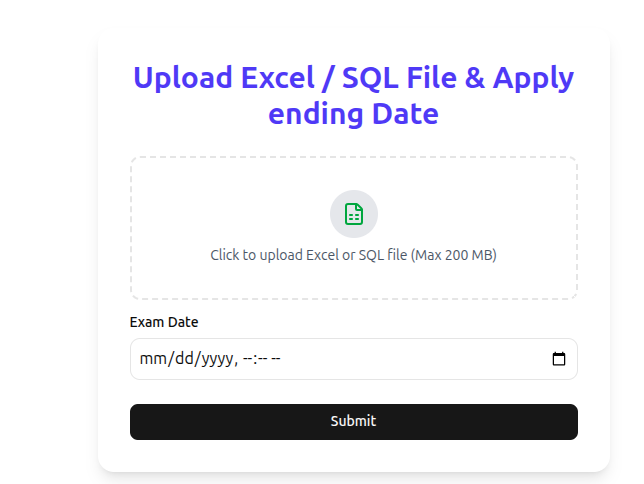
\includegraphics[width=0.75\textwidth]{chapters/chapter4/images/excelupload.png}
    \caption{Excel/SQL File Upload and Application Deadline Interface}
    \label{fig:excel_upload}
\end{figure}

\begin{itemize}
    \item \textbf{Data Ingestion:} The system parses the uploaded file and updates the applicant records. The interface also allows setting an "Exam Date" as a deadline.
    \item \textbf{Cloud Backup:} Using the interface shown in \textit{uploadDrive.png} (if applicable), the admin can sync local data with Google Drive for disaster recovery.
\end{itemize}

\subsection{Examination Announcement}
The admin defines the specific admission unit and the corresponding examination date to notify the applicants.

\begin{figure}[H]
    \centering
    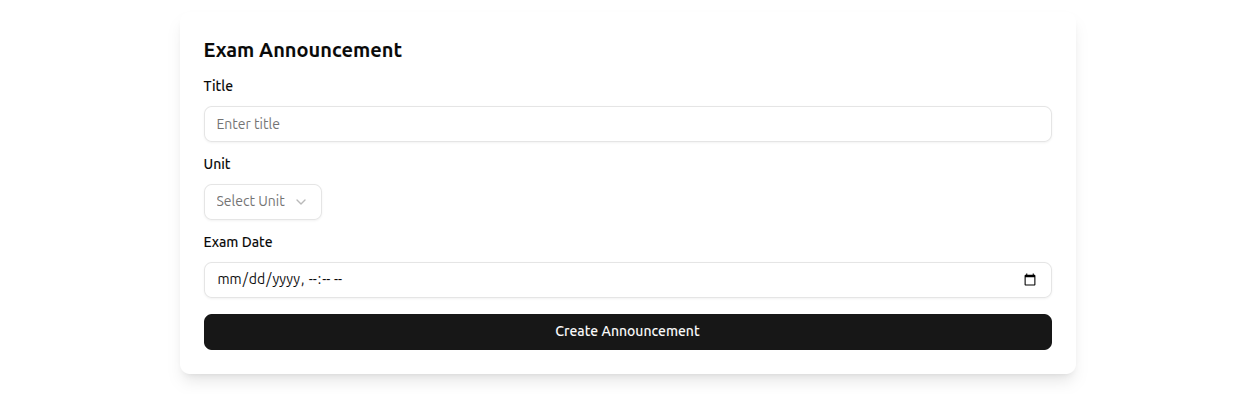
\includegraphics[width=0.75\textwidth]{chapters/chapter4/images/examAnoucement.png}
    \caption{Exam Announcement Configuration Interface}
    \label{fig:exam_announcement}
\end{figure}